\documentclass[acmsmall,screen, nonacm]{acmart}
\usepackage{graphicx}
%%
%% \BibTeX command to typeset BibTeX logo in the docs
\AtBeginDocument{%
  \providecommand\BibTeX{{%
    Bib\TeX}}}

\begin{document}

\title{COSC 520 Assignment 1: Login Search Problem}

\author{Rishav Banerjee}
\email{rishavb@student.ubc.ca}
\affiliation{%
	\institution{University of British Columbia}
	\country{Canada}
}

\renewcommand{\shortauthors}{Banerjee}

%%
%% The abstract is a short summary of the work to be presented in the
%% article.
\begin{abstract}
	An overview of the login search problem, comparing various algorithms.
	The approaches profiled are (1) Linear Search, (2) Binary Search, (3) Hashmap Search, (4) Bloom Filters, and (5) Cuckoo Filters
\end{abstract}
\received{03 October 2025}

%%
%% This command processes the author and affiliation and title
%% information and builds the first part of the formatted document.
\maketitle

\section{Introduction}
The login checker problem involves verifying whether a given username exists within a set of registered usernames.
Efficiently solving this problem is crucial for systems requiring rapid authentication processes.
Various data structures offer different trade-offs in terms of time complexity, space efficiency, and functionality.
This assignment explores several approaches to address the login checker problem.
All code for the assignment can be found on \url{https://github.com/ThatAmuzak/COSC-520-Assignments}, in the \texttt{Assignment-1} directory.

\section{Approaches}

\subsection{Linear Search}
Linear search assignment sequentially checking each username in the list until a match is found or the end is reached.
While simple to implement, its time complexity is \(O(n)\), making it inefficient for large datasets.
The space complexity is \(O(1)\), as it does not require additional memory beyond the input list.
Linear search is particularly useful when the dataset is small or unsorted, and when the position of the username is also required.

\subsection{Binary Search}
Binary search operates on a sorted list by repeatedly dividing the search interval in half.
If the value of the search key is less than the item in the middle of the interval, the search continues in the lower half, or if the value is greater, it continues in the upper half.
This method has a time complexity of \(O(\log n)\) and a space complexity of \(O(1)\).
Binary search is efficient for large, sorted datasets but requires the list to be sorted beforehand, which can incur additional preprocessing time.

\subsection{Hashmaps}
Hashmaps store key-value pairs and allow for average-case constant time complexity \(O(1)\) for lookups, insertions, and deletions.
They achieve this by using a hash function to compute an index into an array of buckets or slots, from which the desired value can be found.
The space complexity is \(O(n)\), where \(n\) is the number of keys.
Hashmaps are highly efficient for checking the existence of a username but do not maintain any order of elements, and their performance can degrade if the hash function leads to many collisions.

\subsection{Bloom Filters}
Bloom filters are probabilistic data structures that test whether an element is a member of a set.
They allow for false positives but not false negatives.
The time complexity for both insertion and lookup operations is \(O(k)\), where \(k\) is the number of hash functions used, and the space complexity is \(O(m)\), where \(m\) is the size of the bit array.
Bloom filters are space-efficient and fast but cannot provide the position of the username and do not support deletion of elements.

\subsection{Cuckoo Filters}
Cuckoo filters~\cite{fan2014Cuckoo} are a variant of Bloom filters that use cuckoo hashing to resolve hash collisions.
They support deletions and provide a bounded false positive rate.
The time complexity for insertion and lookup operations is \(O(1)\), and the space complexity is \(O(n)\), where \(n\) is the number of keys.
Cuckoo filters offer advantages over Bloom filters by allowing deletions and providing better space efficiency in certain scenarios, but they are more complex to implement.

\section{Implementation}
In this section, we describe how each of the approaches to the login checker problem were implemented in Python.
All approaches have been unit tested for validity.

\subsection{Linear Search}
Linear search was implemented by iterating through a Python list and comparing each element with the target username.
If a match is found, the function returns \texttt{True}; otherwise, it returns \texttt{False} after traversing the entire list.
This straightforward approach requires no additional memory beyond the input list.

\subsection{Binary Search}
Binary search was implemented on a sorted Python list.
The search repeatedly calculates the midpoint of the current interval and compares the target with the middle element.
If the target matches, the function returns \texttt{True}.
Otherwise, it continues searching in the appropriate half until the interval is empty.
This method is efficient but requires the list to be sorted beforehand.

\subsection{Hash Table Search}
Hash table search was implemented using Python dictionaries.
The hash table maps each username to its index in the list, allowing constant-time lookups.
Searching involves checking whether the target key exists in the dictionary, returning \texttt{True} if it does.
This approach is fast but consumes additional memory proportional to the number of usernames.

\subsection{Bloom Filter}
The Bloom filter was implemented using the \texttt{bitarray} package and multiple hash functions from \texttt{mmh3}.
Elements are added by hashing them with several hash functions and setting the corresponding bits in the bit array.
Checking membership involves verifying that all corresponding bits are set.
This probabilistic structure is space-efficient and fast but allows for false positives and does not store exact indices.

\subsection{Cuckoo Filter}
The Cuckoo filter was implemented using a compact bitarray representation with two hash functions per element.
Insertion may relocate existing fingerprints to accommodate new elements, and deletion is supported.
Membership checks verify whether the element's fingerprint exists in one of two possible buckets.
This structure is space-efficient, allows deletions, and provides a bounded false positive rate, but is more complex than Bloom filters.

\section{Profiling Methodology}

To evaluate the performance of each search approach for the login checker problem, we implemented a systematic profiling process in Python.
The profiling aimed to measure execution time under both successful and unsuccessful searches across varying dataset sizes.

\subsection{Dataset Generation}
Unique usernames were generated using a simple deterministic scheme, producing strings in the format \texttt{user0, user1, ..., userN-1}.
The maximum dataset size was set according to the largest size in the profiling series, and smaller subsets were sliced from this master list for consistency.
This ensured that all search approaches were tested on identical input datasets.
A maximum size of $10,000,000$ was possible due to out of memory errors beyond that size.

\subsection{Warmup and Timing Strategy}
Each search function underwent a warmup phase before measurements, consisting of \texttt{WARMUP\_COUNT = 3} executions per target.
This warmup allows Python's runtime and CPU branch prediction to stabilize, mitigating artifacts from initial cache misses and interpreter optimizations.

For timing, each search operation was executed \texttt{PER\_REPETITION\_STMT\_COUNT = 5} times per repetition, and the process was repeated \texttt{REPEAT\_COUNT = 10} times.
This procedure produces a distribution of execution times from which minimum, maximum, mean, and standard deviation could be calculated for each dataset size.

\subsection{Search Function Profiling}
\begin{itemize}
	\item \textbf{Linear Search:} Each subset of the dataset was scanned sequentially, comparing elements with the target username.
	\item \textbf{Binary Search:} Conducted on sorted subsets, repeatedly halving the search interval to locate the target.
	\item \textbf{Hashmap Search:} A dictionary mapping usernames to indices was precomputed, enabling constant-time lookups.
	\item \textbf{Bloom Filter:} A bit array with multiple hash functions was initialized, and all usernames were added before measuring membership queries.
	\item \textbf{Cuckoo Filter:} A compact bit array with cuckoo hashing was constructed, supporting insertion of usernames and membership checks.
\end{itemize}

\subsection{Target Selection}
For each dataset size, two scenarios were profiled:
\begin{enumerate}
	\item \textbf{Hit:} The target username is guaranteed to exist in the subset.
	\item \textbf{Miss:} A string that does not exist in the subset is used as the target.
\end{enumerate}
Random seed \texttt{RANDOM\_SEED = 42} was fixed to ensure reproducibility of the selected targets.

\subsection{Metrics Captured}
For each combination of search function, dataset size, and target type (hit/miss), the following metrics were recorded:
\begin{itemize}
	\item Minimum execution time across repetitions
	\item Maximum execution time
	\item Mean execution time
	\item Standard deviation
\end{itemize}
All raw timing results were stored in a pandas DataFrame and exported to a CSV file for further analysis.

\section{Results}

\begin{figure}[H]
	\centering
	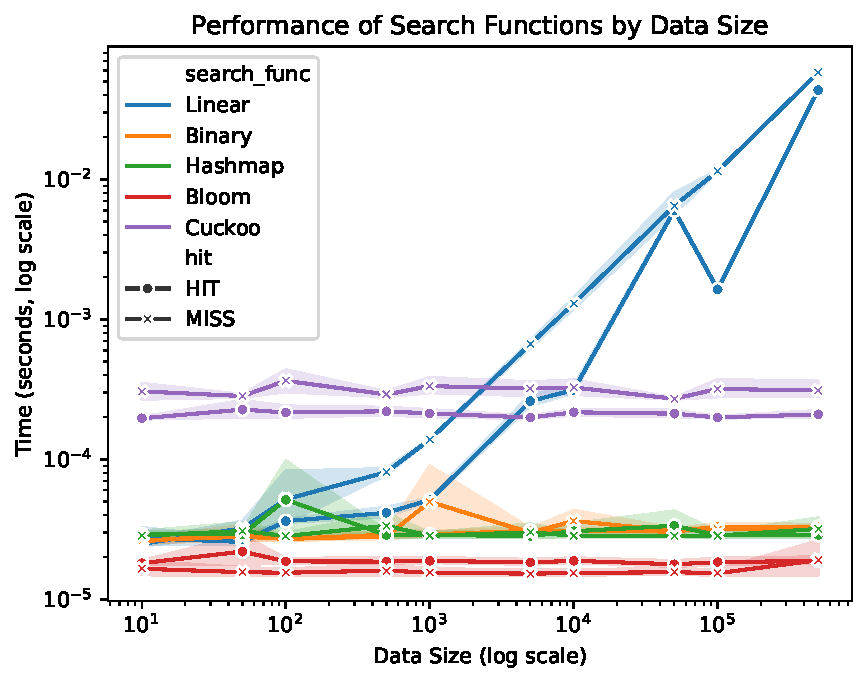
\includegraphics[width=1\textwidth]{results.pdf}
	\caption{Results showcasing the performance of the different functions, with 95\% confidence intervals in the shaded area. The color indicates the search function utilized, while the style of the line indicates if the search performed was using a target present in the relevant data structure (HIT) or not (MISS)}
	\Description{Results showcasing the performance of the different functions, with 95\% confidence intervals in the shaded area. The color indicates the search function utilized, while the style of the line indicates if the search performed was using a target present in the relevant data structure (HIT) or not (MISS)}
	\label{fig:pdfimage}
\end{figure}

The main takeaways from here seem to be as follows:
\begin{enumerate}
	\item Linear time complexities can clearly be observed scaling inefficiently with increasing search spaces
	\item The worst case time complexity (when searching for an element not present) only sometimes outscales the average case time complexity
	\item Cuckoo filters have a constant time overhead which causes a slight loss in performance, but nothing as severe as linear search
\end{enumerate}

\section{Resources}

The following resources were utilized for implementation:
\begin{enumerate}
	\item \href{https://techtonics.medium.com/bloom-filters-your-guide-to-high-performance-data-structures-4db4df3a7838}{Bloom Filters Explained}
	\item \href{https://techtonics.medium.com/implementing-bloom-filters-in-python-and-understanding-its-error-probability-a-step-by-step-guide-13c6cb2e05b7}{Bloom Filters in Python}
	\item \href{https://brilliant.org/wiki/cuckoo-filter/}{Cuckoo Filters Explained}
	\item \href{https://github.com/huydhn/cuckoo-filter}{Cuckoo Filters in Python}
\end{enumerate}




\section{GenAI Usage}
Generative AI was utilized to assist with documentation purposes for the code, and verify code implementations.
All outputs have been manually verified for validity.

\bibliographystyle{ACM-Reference-Format}
\bibliography{sample-base}

\end{document}
\endinput
